%% 
%% Copyright 2019-2020 Elsevier Ltd
%% 
%% This file is part of the 'CAS Bundle'.
%% --------------------------------------
%% 
%% It may be distributed under the conditions of the LaTeX Project Public
%% License, either version 1.2 of this license or (at your option) any
%% later version.  The latest version of this license is in
%%    http://www.latex-project.org/lppl.txt
%% and version 1.2 or later is part of all distributions of LaTeX
%% version 1999/12/01 or later.
%% 
%% The list of all files belonging to the 'CAS Bundle' is
%% given in the file `manifest.txt'.
%% 
%% Template article for cas-dc documentclass for 
%% double column output.

\makeatletter
\def\input@path{{class/}}
\makeatother

%\documentclass[a4paper,fleqn,longmktitle]{cas-dc}
\documentclass[a4paper,fleqn]{cas-dc}

%\usepackage[numbers]{natbib}
%\usepackage[authoryear]{natbib}
\usepackage[authoryear,longnamesfirst]{natbib}

%For full spanning figure
\usepackage{subcaption}
\usepackage{graphicx}
\usepackage{minted}
\usepackage{pdfpages}
\usepackage{xurl}


\usepackage{xcolor}
\usepackage{amsmath,amssymb,tabularray}
% Global CUDAHeat colour palette. Load after xcolor.
% Palette combines accessible categorical colours with ocean/thermal ramps.

% Brand and categorical colours.
\definecolor{CUDAHeatNavy}{HTML}{003B5C}
\definecolor{CUDAHeatBlue}{HTML}{0072B2}
\definecolor{CUDAHeatSky}{HTML}{56B4E9}
\definecolor{CUDAHeatTeal}{HTML}{009E73}
\definecolor{CUDAHeatGreen}{HTML}{3A923A}
\definecolor{CUDAHeatLime}{HTML}{7CB342}
\definecolor{CUDAHeatGold}{HTML}{F0E442}
\definecolor{CUDAHeatYellow}{HTML}{E69F00}
\definecolor{CUDAHeatOrange}{HTML}{D55E00}
\definecolor{CUDAHeatVermilion}{HTML}{C84E00}
\definecolor{CUDAHeatMagenta}{HTML}{CC79A7}
\definecolor{CUDAHeatPurple}{HTML}{7A5195}

% Ocean ramp.
\definecolor{OceanPale}{HTML}{F7FBFF}
\definecolor{OceanMist}{HTML}{DEEBF7}
\definecolor{OceanLight}{HTML}{C6DBEF}
\definecolor{OceanBlue}{HTML}{6BAED6}
\definecolor{OceanDeep}{HTML}{2171B5}
\definecolor{OceanAbyss}{HTML}{08306B}

% Thermal ramp.
\definecolor{ThermalPale}{HTML}{FFF5F0}
\definecolor{ThermalBlush}{HTML}{FEE0D2}
\definecolor{ThermalCoral}{HTML}{FCBBA1}
\definecolor{ThermalSalmon}{HTML}{FC6A4A}
\definecolor{ThermalRed}{HTML}{DE2D26}
\definecolor{ThermalMaroon}{HTML}{67000D}

% Neutral and document colours.
\definecolor{CUDAHeatInk}{HTML}{1F2933}
\definecolor{CUDAHeatCharcoal}{HTML}{3E4C59}
\definecolor{CUDAHeatSlate}{HTML}{627D98}
\definecolor{CUDAHeatSteel}{HTML}{9FB3C8}
\definecolor{CUDAHeatGrid}{HTML}{D9E2EC}
\definecolor{CUDAHeatMist}{HTML}{F0F4F8}
\definecolor{CUDAHeatPaper}{HTML}{FFFFFF}

% Semantic pipeline colours used by TikZ/PGFPlots figures.
\colorlet{PipelineDiskCPU}{CUDAHeatBlue}
\colorlet{PipelineCPUGPU}{CUDAHeatSky}
\colorlet{PipelineCompute}{CUDAHeatTeal}
\colorlet{PipelineGPUCPU}{CUDAHeatOrange}

% Semantic time-series colours. Use these names in every event figure.
\colorlet{SSTLine}{CUDAHeatInk}
\colorlet{ClimatologyLine}{CUDAHeatBlue}
\colorlet{ThresholdLine}{ThermalRed}
\colorlet{EventShade}{CUDAHeatGold!24}

% Tables, rules, and source-code blocks.
\colorlet{RuleBlue}{CUDAHeatBlue}
\definecolor{codebg}{HTML}{F7F7F7}
\definecolor{codeframe}{HTML}{D0D0D0}
\definecolor{terminalbg}{HTML}{1E1E1E}
\definecolor{terminalfg}{HTML}{E6E6E6}

\definecolor{header}{HTML}{24384F}
\definecolor{ruleline}{HTML}{CAD4DE}
\definecolor{metadata}{HTML}{5B6B7C}
\definecolor{rowshade}{HTML}{F3F6F8}
\hypersetup{hidelinks}
\usepackage{tabularx}
% Preamble
\usepackage{booktabs}
\usepackage{tabularx}
\usepackage{array}

\newcolumntype{Y}{>{\raggedright\arraybackslash}X}
\urlstyle{tt}
\newcommand{\code}[1]{\nolinkurl{#1}}
\setlength{\parindent}{0pt}


\setminted[python]{
    fontsize=\scriptsize,
    breaklines=true,
    autogobble=true,
    linenos=true,
    numbersep=6pt,
    frame=single,
    framesep=2mm,
    rulecolor=\color{codeframe},
    bgcolor=codebg,
    style=friendly
}

\setminted[text]{
    fontsize=\scriptsize,
    breaklines=true,
    autogobble=true,
    frame=single,
    framesep=2mm,
    rulecolor=\color{codeframe},
    bgcolor=terminalbg,
    style=friendly
}

\usepackage{stfloats}
\usepackage{pdflscape}
\usepackage{tikz}
\usepackage{pgfplots}
    \usetikzlibrary{
        pgfplots.dateplot,
    }



\pgfplotsset{compat=1.18}
\usepgfplotslibrary{polar}
\usetikzlibrary{calc}

\pgfplotsset{
    colormap={mhwred}{
        rgb255(0cm)=(255,245,240);
        rgb255(1cm)=(254,224,210);
        rgb255(2cm)=(252,187,161);
        rgb255(3cm)=(252,106,74);
        rgb255(4cm)=(222,45,38);
        rgb255(5cm)=(103,0,13)
    },
    colormap={climblue}{
        rgb255(0cm)=(247,251,255);
        rgb255(1cm)=(222,235,247);
        rgb255(2cm)=(198,219,239);
        rgb255(3cm)=(107,174,214);
        rgb255(4cm)=(49,130,189);
        rgb255(5cm)=(8,48,107)
    }
}

%%%Author definitions
\def\tsc#1{\csdef{#1}{\textsc{\lowercase{#1}}\xspace}}
\tsc{WGM}
\tsc{QE}
\tsc{EP}
\tsc{PMS}
\tsc{BEC}
\tsc{DE}
%%%


\begin{document}
\let\WriteBookmarks\relax
\def\floatpagepagefraction{1}
\def\textpagefraction{.001}

% Short title
\shorttitle{Marine Heat Waves and hoyurly scale}

% Short author
\shortauthors{M. Miani et~al.}

% Main title of the paper
\title [mode = title]{From Daily to Hourly Marine Heatwaves: A Taxonomy-Based, GPU-Accelerated Framework for Event Detection and Classification} 
                   
% Title footnote mark
% eg: \tnotemark[1]
%\tnotemark[1,2]

% Title footnote 1.
% eg: \tnotetext[1]{Title footnote text}
% \tnotetext[<tnote number>]{<tnote text>} 
\tnotetext[1]{"This project has received funding from the European Union’s Horizon 2020 research and innovation programme under grant agreement No. 856612 and the Cyprus Government."}




\author[1]{Marco Miani}[%
    orcid=0000-0003-4136-9640
]
\cormark[1]
\ead{m.miani@cyi.ac.cy}
\credit{Conceptualization, Methodology, Software, Writing - Original draft}


\author[1]{Panos Hadjinicolaou}
\credit{Supervision, Methodology, Writing - Review \& Editing}

\author[1]{Yiannis Proestos}
\credit{Supervision, Methodology, Writing - Review \& Editing}

\author[1,2]{Jos Lelieveld}
\credit{Supervision, Writing - Review \& Editing}

\author[3]{Nadia Pinardi}
\credit{Methodology, Writing - Review \& Editing}



\affiliation[1]{organization={The Cyprus Institute},
    addressline={20 Konstantinou Kavafi Street},
    city={Nicosia},
    postcode={2121},
    country={Cyprus}
}


\affiliation[2]{organization={Max-Planck-Insitut},
    addressline={Hahn-Meitner-Weg, 1},
    city={Mainz},
    postcode={55128},
    country={Germany}
}

\affiliation[3]{organization={CMCC Foundation - Euro-Mediterranean Center on Climate Change},
    addressline={},
    city={},
    postcode={},
    country={Italy}
}


% Here goes the abstract
\begin{abstract}
\noindent This study presents a methodology for detecting, analysing, and classifying Marine heatwaves (MHWs) at hourly resolution. 
MHWs are traditionally identified from daily Sea Surface Temperature (SST)
records, yet this framework does not transfer directly to higher temporal resolution. At hourly scale,
SST reveals sub-daily variability that is largely smoothed out in daily means, including intermittent
threshold exceedances, short-lived interruptions, diurnal cycling, and nocturnal heat retention. These
features complicate the definition of event continuity and persistence, but also provide an opportunity
to examine the internal structure of marine heat extremes in substantially greater detail.

\noindent 
Events are identified through a duration--gap framework that preserves short interruptions while
maintaining event continuity, and are subsequently decomposed into individual diurnal cycles. Their
intra-event morphology is used to construct an hourly-scale taxonomy that characterises MHWs not only
in terms of conventional duration and intensity, but also through persistence, interruption structure,
cycle-to-cycle evolution, diurnal heating, nocturnal retention, and other sub-daily dynamics that are
not accessible from daily observations. To enable the methodology to scale from individual time
series to multi-year gridded SST datasets, a GPU-accelerated implementation, \texttt{CUDAHeat}, is
developed using CUDA-enabled array computation. The computational architecture preserves the complete
temporal record of each spatial point while partitioning only the spatial domain into dynamically sized
batches according to available GPU memory. VRAM-aware batch adaptation, automatic out-of-memory
recovery, and explicit support for both 32-bit and 64-bit floating-point computation allow the same
workflow to operate across different GPU memory capacities without altering the temporal definition
of an event.

\noindent Benchmarking on a hourly gridded SST dataset comprising approximately 1.16 billion values
shows a $23.4\times$ acceleration of the core computation using GPU 32-bit arithmetic relative to the
CPU 64-bit reference, with a $15.9\times$ speedup for the complete processing pipeline. Scientific
validation yields approximately $99.9991\%$ agreement in threshold-exceedance classification across
tens of millions of comparisons, with the remaining differences confined predominantly to values
extremely close to the detection threshold. These results demonstrate that the hourly framework can
retain its temporal and taxonomic detail while remaining computationally tractable for substantially
larger spatial datasets. This combination of an hourly event taxonomy with scalable GPU computation provides a framework for
investigating marine heat extremes from their conventional daily representation down to their
sub-daily structure, and establishes a basis for subsequent analysis of coupled marine--atmospheric
heat extremes and coastal thermal stress.
\end{abstract}





% Keywords
% Each keyword is seperated by \sep
\begin{keywords}
MHWs, SST, GPU, Taxonomy
\end{keywords}


\maketitle

\tableofcontents
\clearpage

\section{Introduction}

\subsection{Marine Heatwaves and Temporal Resolution}

Marine heatwaves are commonly defined as discrete intervals during which sea-surface temperature (SST) exceeds a seasonally varying local threshold for a prescribed minimum duration \citep{Hobday2016}. This event-based formulation has enabled coherent assessment of changes in the frequency, duration and intensity of marine thermal extremes at global scale \citep{Oliver2018}. Its conventional implementation, however, is predominantly based on daily SST products. Daily aggregation is scientifically useful for synoptic-to-seasonal analyses, but it suppresses the temporal structure that governs threshold crossing at sub-daily resolution.

At hourly resolution, a thermal anomaly is not a single daily value but a trajectory that may cross the climatological threshold repeatedly within one diurnal cycle. The timing, persistence and ordering of these crossings contain information about daytime warming, nocturnal recovery, transient interruption and event continuity. An hourly framework must therefore preserve the full temporal sequence while distinguishing physically meaningful short interruptions from changes in event state. This requirement motivates an event-detection formulation in which the climatological reference, threshold construction and temporal morphology are all resolved at the sampling interval of the observations.

\subsection{Scope of This Work}

This article presents CUDAHeat, a GPU-native Python framework for hourly SST climatology, event detection relative to a threshold, sparse event representation and rule-based event enrichment. The framework translates the conceptual hierarchy of marine-heatwave detection to gridded hourly data while retaining the complete time series at every spatial location. The emphasis is methodological: the objective is to provide a reproducible and inspectable route from SST input data to event catalogues and taxonomic descriptors, rather than to prescribe a universal set of ecological or regional thresholds.

The manuscript first defines the rationale for resolving marine heatwaves at hourly cadence, then describes the numerical methodology, software implementation and enrichment architecture. Results are expressed as the scientific and computational products of the workflow: timestamp-resolved thresholds, sparse event intervals and event-aligned descriptors that support subsequent regional or process-based analysis.

\subsection{Why hourly SST Data?}

Hourly observations resolve the diurnal cycle as part of the local climatological signal rather than as residual variability. The relevant comparison is therefore between an observation and a threshold for the same calendar phase and clock hour, not between an hourly observation and a daily reference. This enables event descriptors to distinguish, for example, frequent strong daytime exceedances from persistent nocturnal threshold retention. Such descriptors are complementary to conventional duration and intensity metrics: they describe the temporal organisation of thermal stress within an event.

The increased resolution also requires a more explicit treatment of continuity. Short sequences below threshold may reflect a physically relevant interruption, an observation gap or the expected nightly phase of a diurnal cycle. CUDAHeat represents these alternatives through independently specified internal-gap and joining rules, so that the analytical assumptions are visible in the event metadata rather than being embedded implicitly in temporal aggregation.


\subsection{CUDAHeat}

\subsubsection{Purpose and Scope}

CUDAHeat is designed for gridded SST records in which the temporal dimension is complete and regularly sampled at hourly resolution. It computes a seasonally and diurnally resolved climatology, derives a percentile threshold, identifies threshold-exceedance events and returns their compact catalogue. The package also exposes the climatology, threshold and exceedance fields for applications whose output domain is sufficiently small to be held in host memory. The implementation accepts a NetCDF path or an already-open \code{xarray.Dataset}; the principal public object is \code{CUDAHeat}.

The package separates three scientific products. First, the climatological cycle and percentile threshold constitute the reference state against which an observation is evaluated. Second, the detector converts the instantaneous exceedance relation into time intervals after explicitly applying rules for short internal gaps, minimum duration and event joining. Third, an optional enrichment stage calculates event-level quantities from versioned YAML rules. This separation avoids conflating the definition of an event with the metrics subsequently used to characterise it.

\subsubsection{Design Principles}

The central computational invariant is that CUDAHeat never partitions a time series. Spatial dimensions are stacked into a point dimension, and each GPU operation receives an array of shape $(T, P_b)$, where $T$ is the complete number of time steps and $P_b$ is the active spatial batch. Preserving $T$ is essential because temporal segmentation at batch boundaries would alter circular climatology, duration counting and gap logic. When memory is limiting, the package reduces only $P_b$; if a single complete time series cannot fit on the selected device, execution terminates with an explicit memory error rather than silently changing the analysis.

%Numerical operations are expressed against an array backend so that the same vectorized formulation can be evaluated with CuPy on the GPU and with NumPy for reference calculations. 
The production default is \code{float32}, whereas \code{float64} remains available when the precision requirements of a particular data product warrant the additional memory cost. Missing values are retained as missing throughout the climatological calculation and cannot be classified as threshold exceedances.

\subsubsection{Processing Workflow}

The standard workflow begins by preparing the input layout and resolving the temporal coordinate. CUDAHeat then assigns each timestamp to an hourly climatology bin, selects the requested baseline, estimates the climatological mean and percentile threshold, and aligns these cycles to the complete record. Detection produces a sparse catalogue indexed by spatial point and half-open time interval. The catalogue may be queried directly, reconstructed lazily as a dense event-ID field, or passed to the enrichment subsystem. This workflow makes the threshold definition, detection parameters, input preparation and enrichment provenance available as structured metadata alongside the event product.

\section{CUDAHeat}

\subsection{Purpose and Scope}

CUDAHeat is designed for gridded SST records in which the temporal dimension is complete and regularly sampled at hourly resolution. It computes a seasonally and diurnally resolved climatology, derives a percentile threshold, identifies threshold-exceedance events and returns their compact catalogue. The package also exposes the climatology, threshold and exceedance fields for applications whose output domain is sufficiently small to be held in host memory. The implementation accepts a NetCDF path or an already-open \code{xarray.Dataset}; the principal public object is \code{CUDAHeat}.

The package separates three scientific products. First, the climatological cycle and percentile threshold constitute the reference state against which an observation is evaluated. Second, the detector converts the instantaneous exceedance relation into time intervals after explicitly applying rules for short internal gaps, minimum duration and event joining. Third, an optional enrichment stage calculates event-level quantities from versioned YAML rules. This separation avoids conflating the definition of an event with the metrics subsequently used to characterise it.

\subsection{Design Principles}

The central computational invariant is that CUDAHeat never partitions a time series. Spatial dimensions are stacked into a point dimension, and each GPU operation receives an array of shape $(T, P_b)$, where $T$ is the complete number of time steps and $P_b$ is the active spatial batch. Preserving $T$ is essential because temporal segmentation at batch boundaries would alter circular climatology, duration counting and gap logic. When memory is limiting, the package reduces only $P_b$; if a single complete time series cannot fit on the selected device, execution terminates with an explicit memory error rather than silently changing the analysis.

Numerical operations are expressed against an array backend so that the same vectorized formulation can be evaluated with CuPy on the GPU and with NumPy for reference calculations. The production default is \code{float32}, whereas \code{float64} remains available when the precision requirements of a particular data product warrant the additional memory cost. Missing values are retained as missing throughout the climatological calculation and cannot be classified as threshold exceedances.

\subsection{Processing Workflow}

The standard workflow begins by preparing the input layout and resolving the temporal coordinate. CUDAHeat then assigns each timestamp to an hourly climatology bin, selects the requested baseline, estimates the climatological mean and percentile threshold, and aligns these cycles to the complete record. Detection produces a sparse catalogue indexed by spatial point and half-open time interval. The catalogue may be queried directly, reconstructed lazily as a dense event-ID field, or passed to the enrichment subsystem. This workflow makes the threshold definition, detection parameters, input preparation and enrichment provenance available as structured metadata alongside the event product.

\section{Why Move from Daily to Hourly Data}

\subsection{Limitations of Daily Aggregation}

Daily averaging is a temporal filter. It can reduce the influence of retrieval noise and provide a natural representation of persistent weather-scale anomalies, but it also combines daytime heating and nocturnal cooling into a single statistic. A daily mean may remain below a daily threshold despite a sustained daytime exceedance, or may remain above it while part of the diurnal cycle is below the appropriate hourly threshold. Consequently, the event boundary inferred from daily data is not generally equivalent to the boundary inferred from the underlying hourly series.

This distinction is particularly consequential near event onset and termination. At these transitions, the classification of a small number of hours can determine whether adjacent periods form one event or several events. The loss of phase information also prevents a direct assessment of whether thermal persistence is maintained overnight, whether extremes are concentrated near the daytime maximum, or whether a nominally continuous warm period contains recurrent sub-daily interruptions.

\subsection{Sub-Daily Marine Heatwave Dynamics}

Hourly observations resolve the diurnal cycle as part of the local climatological signal rather than as residual variability. The relevant comparison is therefore between an observation and a threshold for the same calendar phase and clock hour, not between an hourly observation and a daily reference. This enables event descriptors to distinguish, for example, frequent strong daytime exceedances from persistent nocturnal threshold retention. Such descriptors are complementary to conventional duration and intensity metrics: they describe the temporal organisation of thermal stress within an event.

The increased resolution also requires a more explicit treatment of continuity. Short sequences below threshold may reflect a physically relevant interruption, an observation gap or the expected nightly phase of a diurnal cycle. CUDAHeat represents these alternatives through independently specified internal-gap and joining rules, so that the analytical assumptions are visible in the event metadata rather than being embedded implicitly in temporal aggregation.

\subsection{Hourly Data Requirements}

The input time coordinate must be contiguous at hourly spacing. The framework validates this condition before detection because the duration and gap parameters are expressed in hours and are meaningful only on a regular time axis. SST values may contain \code{NaN}s; they are excluded from climatological statistics and do not satisfy the exceedance relation. The resulting event interpretation remains conditional on the observational product, including its retrieval physics, spatial resolution, gap structure and local-time convention. For gridded reconstructions of hourly SST, these considerations should be assessed before comparing event statistics across regions or data products \citep{Marullo2014}.

\section{Methodology}

\subsection{Data Preparation}



CUDAHeat accepts a NetCDF source path or an \code{xarray.Dataset} containing the selected SST variable. The temporal coordinate is resolved explicitly and validated as a contiguous hourly sequence. All non-temporal dimensions are treated as spatial dimensions and are stacked into a single point axis for computation. This transformation is representational rather than analytical: point coordinates and the original grid indexing are retained so that event products can be returned in their native spatial geometry.
For path-based inputs, the package can construct or reuse a validated compact time-by-point NetCDF representation. The cache is held outside the source file and is identified by source and storage metadata, thereby preventing reuse after incompatible source changes. This optimization improves the regularity of spatial reads without modifying the scientific time axis. Inputs already arranged in time-by-point form are used directly; alternatively, users may bypass or require optimization explicitly.

\subsection{Hourly Climatology and Threshold Estimation}



Let $S(t,p)$ denote SST at time $t$ and point $p$. A baseline interval selects the rows used to estimate the reference cycle. Under the default \code{month_day_hour} calendar, each timestamp is assigned to one of $366\times24$ bins, preserving calendar date and clock hour. A \code{dayofyear} mode is also available. The default construction follows an hourly extension of the seasonal-threshold approach: for each calendar day and clock hour, samples from the same clock hour within $\pm5$ calendar days of the target day are pooled across the baseline. The climatological mean $C$ and percentile threshold $Q_q$ are calculated from this pool, with $q=0.90$ by default \citep{Hobday2016}.
For the month--day--hour calendar, the initially estimated 29 February bins are interpolated from the surrounding calendar days. This preserves a complete 366-day cycle while avoiding a discontinuity associated with the sparse occurrence of leap-day observations. All statistics are NaN-aware: a bin with no finite support remains missing rather than receiving an imputed temperature.



The raw mean and threshold cycles are circularly smoothed with a 31-day window by default, equivalent to 744 h. Smoothing is applied separately to each clock-hour sequence; it therefore regularizes the seasonal evolution of, for example, 14:00 SST without blending it with the 02:00 climatology. The smoothed cycles are then indexed by the full timestamp sequence to obtain $C(t,p)$ and $Q_q(t,p)$. The corresponding anomaly and exceedance magnitude are $A(t,p)=S(t,p)-C(t,p)$ and $E(t,p)=S(t,p)-Q_q(t,p)$, respectively.

\subsection{Event Detection}



The instantaneous exceedance mask is defined as
\[
M(t,p)=\bigl[S(t,p)>Q_q(t,p)\bigr]\land\bigl[S(t,p)\ \mathrm{is\ finite}\bigr].
\]
The strict inequality is intentional: observations equal to the threshold are not exceedances. A missing SST or threshold cannot generate an exceedance. CUDAHeat retains this raw mask conceptually distinct from the continuity-adjusted mask used to identify candidate intervals, allowing enrichment rules to measure raw thermal behaviour even when event continuity permits short interruptions.



The detector first fills only internal false runs bounded on both sides by exceedances and no longer than \code{max_internal_gap_hours}; the default is 6 h. Maximal true intervals are then extracted from this filled mask and retained when their duration is at least \code{min_duration_hours}, which defaults to 120 h. Finally, neighbouring duration-qualified intervals at the same spatial point are joined when their separating gap does not exceed \code{join_gap_hours}, which defaults to 48 h. The order of these operations is consequential: duration filtering precedes joining, and the joining operation acts on sparse intervals rather than on a dense label field.

The following parameter table summarizes the user-modulable settings that define the hourly reference and the temporal event rule. These values should be treated as an explicit analytical configuration, not as universally transferable constants.

\begin{table*}[t]
\centering
\footnotesize
\renewcommand{\arraystretch}{1.18}
\rowcolors{2}{gray!12}{white}
\begin{tabularx}{\textwidth}{@{}
    p{0.1\textwidth}
    p{0.10\textwidth}
    p{0.2\textwidth}
    X
@{}}
\toprule
Parameter & Default & Permitted setting & Scientific role \\
\midrule
\code{baseline} & \code{None} & \code{None} or \code{(start_year, end_year)} & Selects the observations used to estimate the climatological mean and percentile threshold. \\
\code{percentile} & $0.90$ & $0<q<1$ & Defines the quantile threshold $Q_q(t,p)$. \\
\code{calendar_mode} & \code{month_day_hour} & \code{month_day_hour} or \code{dayofyear} & Determines the assignment of timestamps to hourly climatology bins. \\
\code{smooth_window_hours} & 744 h & Positive 24-h multiple within the annual cycle & Sets the same-clock-hour circular smoothing window. \\
\code{smooth_min_periods} & 1 day & Integer from 1 to the smoothing-window length in days & Sets the minimum finite support required during smoothing. \\
\code{min_duration_hours} & 120 h & Integer $\geq 1$ & Retains candidate intervals at or above the prescribed duration. \\
\code{max_internal_gap_hours} & 6 h & Integer $\geq 0$ & Fills bounded sub-threshold interruptions before duration filtering. \\
\code{join_gap_hours} & 48 h & Integer $\geq 0$ & Joins neighbouring duration-qualified intervals at the same point. \\
\bottomrule
\end{tabularx}
\rowcolors{2}{}{}
\par\vspace{3pt}
\parbox{\textwidth}{\sffamily\small\textbf{Parameter settings.}\enspace User-modulable CUDAHeat parameters governing climatology construction and event detection; values shown are the current defaults.}
\end{table*}

\subsection{Event Representation}



Each retained event is represented as a point index and a half-open interval $[t_{\mathrm{start}},t_{\mathrm{stop}})$, together with duration and associated metadata. This sparse representation is appropriate because marine heatwave occupancy is ordinarily much smaller than the full time--space domain. It also supports direct event filtering by time, location or duration without reconstructing a dense cube.



When a dense representation is required for interoperability, CUDAHeat reconstructs a Dask-backed event-ID field in time chunks. Zero denotes the absence of a retained event and positive integers identify catalogue entries. The reconstruction is deliberately lazy: users can subset or write the result without allocating the full time--space array in host memory. Point-level and event-level accessors additionally provide SST, climatology, threshold and event context for targeted inspection.

\section{Python Implementation}

\subsection{Package Architecture and Public API}

CUDAHeat is implemented as a Python package with a narrow public interface and separable numerical components. \code{core.py} orchestrates input preparation, device execution and result assembly; \code{climatology.py} and \code{detection.py} contain the numerical kernels; \code{result.py} defines sparse event accessors; and \code{enrichment.py} evaluates extensible event rules. The top-level \code{CUDAHeat} class provides \code{run()}, \code{climatology()}, \code{thresholds()}, \code{mask()}, \code{detect()} and \code{validate()} methods. The distinction between generic field production and event detection prevents allocation of full timestamp-aligned fields when only a compact event catalogue is needed.

The software uses CuPy for production GPU arrays but retains a NumPy reference path for numerical diagnostics. Device availability is required when constructing \code{CUDAHeat}, whereas importing the package does not itself require CuPy. This design permits workflows that inspect results, post-process catalogues or validate stored outputs on systems without a CUDA runtime.

\subsection{NetCDF and xarray Input Handling}

The I/O layer resolves the temporal coordinate, identifies spatial dimensions and preserves coordinate information needed to reconstruct the original grid. A source may be opened eagerly or through Dask-backed xarray reads. Lazy I/O constrains host-side read memory; it does not alter the complete-time requirement of the GPU calculation. Each spatial batch still contains every timestamp for its selected points, and data are converted to the explicit analysis precision before device execution.

\subsection{Point-Layout Optimization and Input Caching}

For a conventional gridded NetCDF file, the preprocessing layer can write a compact cache in which spatial dimensions have been stacked into point. The cache is separate from the raw archive and records source identity and layout metadata. It is therefore an optimization of access pattern rather than a replacement scientific data product. The option \code{input_optimization="auto"} uses an existing compatible point layout or prepares one; \code{"skip"} retains direct input handling, whereas \code{"require"} rejects an unoptimized grid.

Compact climatology and threshold cycles can likewise be stored in a Zarr cache for compatible optimized path inputs. The cache contains the small annual-cycle fields rather than a dense timestamp-aligned threshold field, preserving the memory advantage of the cyclic representation. Cache keys incorporate the baseline, percentile, smoothing choices, calendar mode and source metadata so that changes to the analytical definition invalidate reuse.

\subsection{GPU Batching and VRAM Management}

The executor transfers complete-time spatial batches to the selected CUDA device. When \code{batch_size="guess"}, an initial size is selected from a conservative fraction of free VRAM; an explicit positive batch size may also be supplied. A configurable safety reserve, 15\% by default, is retained from currently free memory. If a device out-of-memory exception occurs, the failed batch is released, its spatial width is reduced and the same spatial subset is retried. No time axis is partitioned during this recovery.

Although the API accepts selected device identifiers, the current implementation executes batches sequentially on the first selected device. Telemetry records host read, host preparation, transfer and GPU timings per batch, together with retry information and the active batch size. These diagnostics are operational metadata, not substitutes for scientific validation of the SST product or the event definition.

\subsection{xarray Event Products and PostgreSQL Persistence}

Results are represented as xarray datasets so that event tables, point coordinates and metadata remain interoperable with the scientific Python ecosystem. The optional PostgreSQL layer persists run metadata, spatial-point identities, sparse events and enrichment values. It does not persist the original SST cube or dense climatology arrays. Stored runs include a reproducible fingerprint derived from the detection configuration, source identity and rule catalogue; rule versions and content hashes provide an auditable link between an enrichment output and the executable specification that produced it.

\section{Hourly Marine Heatwave Taxonomy}

\subsection{Taxonomic Framework}

The taxonomic layer is formulated as a set of explicit, event-aligned measurements rather than as a fixed unsupervised classification. This choice preserves interpretability: every descriptor has a declared formula, unit, valid range and implementation. The taxonomy can therefore be expanded as a scientific question changes, while event detection remains stable. Metrics are evaluated over the final event interval and may use raw exceedance, SST, climatology, threshold, temporal indices and spatial coordinates supplied by the rule context.

The current catalogue illustrates complementary dimensions of hourly event structure. Threshold-exceedance fraction quantifies the fraction of valid event hours above the climatological threshold. Daytime strong-exceedance fraction characterises frequent large daytime anomalies relative to the threshold--climatology separation. Heat content integrates positive threshold exceedance through time. Nocturnal below-climatology and below-threshold fractions describe nighttime recovery or interruption. Nocturnal-to-daytime heat retention assesses whether nighttime SST remains above a reference set by the preceding daytime threshold. These descriptors should be interpreted jointly: none is a universal proxy for impact, persistence or cumulative thermal exposure.

\subsection{Feature-Space Representation and Principal Component Analysis}

For multivariate analysis, an event $i$ may be represented as a point in an $N$-dimensional descriptor space,
\[
\mathcal{E}_i = \mathcal{E}\bigl(\tilde{x}_{i1},\tilde{x}_{i2},\ldots,\tilde{x}_{iN}\bigr),
\]
where $x_{ij}$ is the $j$th scalar derived for the event and $\tilde{x}_{ij}$ is its declared normalized form. CUDAHeat returns the raw, physically interpretable scalars; it does not silently normalize descriptors or assign principal components. Normalization is an analysis-stage decision because the appropriate transformation depends on the comparison population, the distribution of each metric and the scientific question. For example, standardization by $\tilde{x}_{ij}=(x_{ij}-\mu_j)/\sigma_j$ is appropriate for principal component analysis (PCA) only when $\mu_j$ and $\sigma_j$ are estimated from a clearly defined event set and variables with zero or near-zero variance are handled explicitly.

PCA can then be applied to the complete, normalized descriptor matrix to identify orthogonal directions of maximal variance. Component scores provide a low-dimensional projection for exploration, whereas loadings identify which standardized descriptors contribute to each component. PCA is descriptive rather than a proof of discrete event types: its interpretation requires reporting the event-selection criteria, transformations, normalization reference set, retained components and explained variance. Missing descriptors should be handled by a declared complete-case or imputation procedure before fitting, rather than being implicitly discarded by plotting software.

\subsection{YAML Rule Catalogues}

Each enrichment rule is a YAML document with a stable identifier, semantic version, short and long names, mathematical formula, symbol definitions, category metadata and output specification. The output specification declares a name, unit, range and dimensions. The rule document also contains a Python \code{calculate} function. At discovery, CUDAHeat validates the schema, rejects duplicate identifiers or output names, compiles the function and records a SHA-256 hash of the source document. This design couples an event variable to its precise mathematical and computational definition.

The explicit formula and symbol metadata are intended to make the taxonomic catalogue suitable for scientific reporting. A rule is not merely a column added to an event table: it is a versioned hypothesis about which aspect of event morphology is informative. The catalogue should consequently be curated with the same care as the detection configuration, including unit consistency, handling of missing values and the physical interpretation of extrema or thresholds.

\subsection{Current Rule Catalogue}

The rule catalogue is presented in Table~\ref{tab:cudaheat-rules}. It is generated directly from the YAML rule specifications in the rule directory and typeset by \code{create_Latex_table.tex}. The catalogue documents the rule symbols, units, formulas, descriptions and interpretations used in the current implementation.

\clearpage
\refstepcounter{table}
\label{tab:cudaheat-rules}
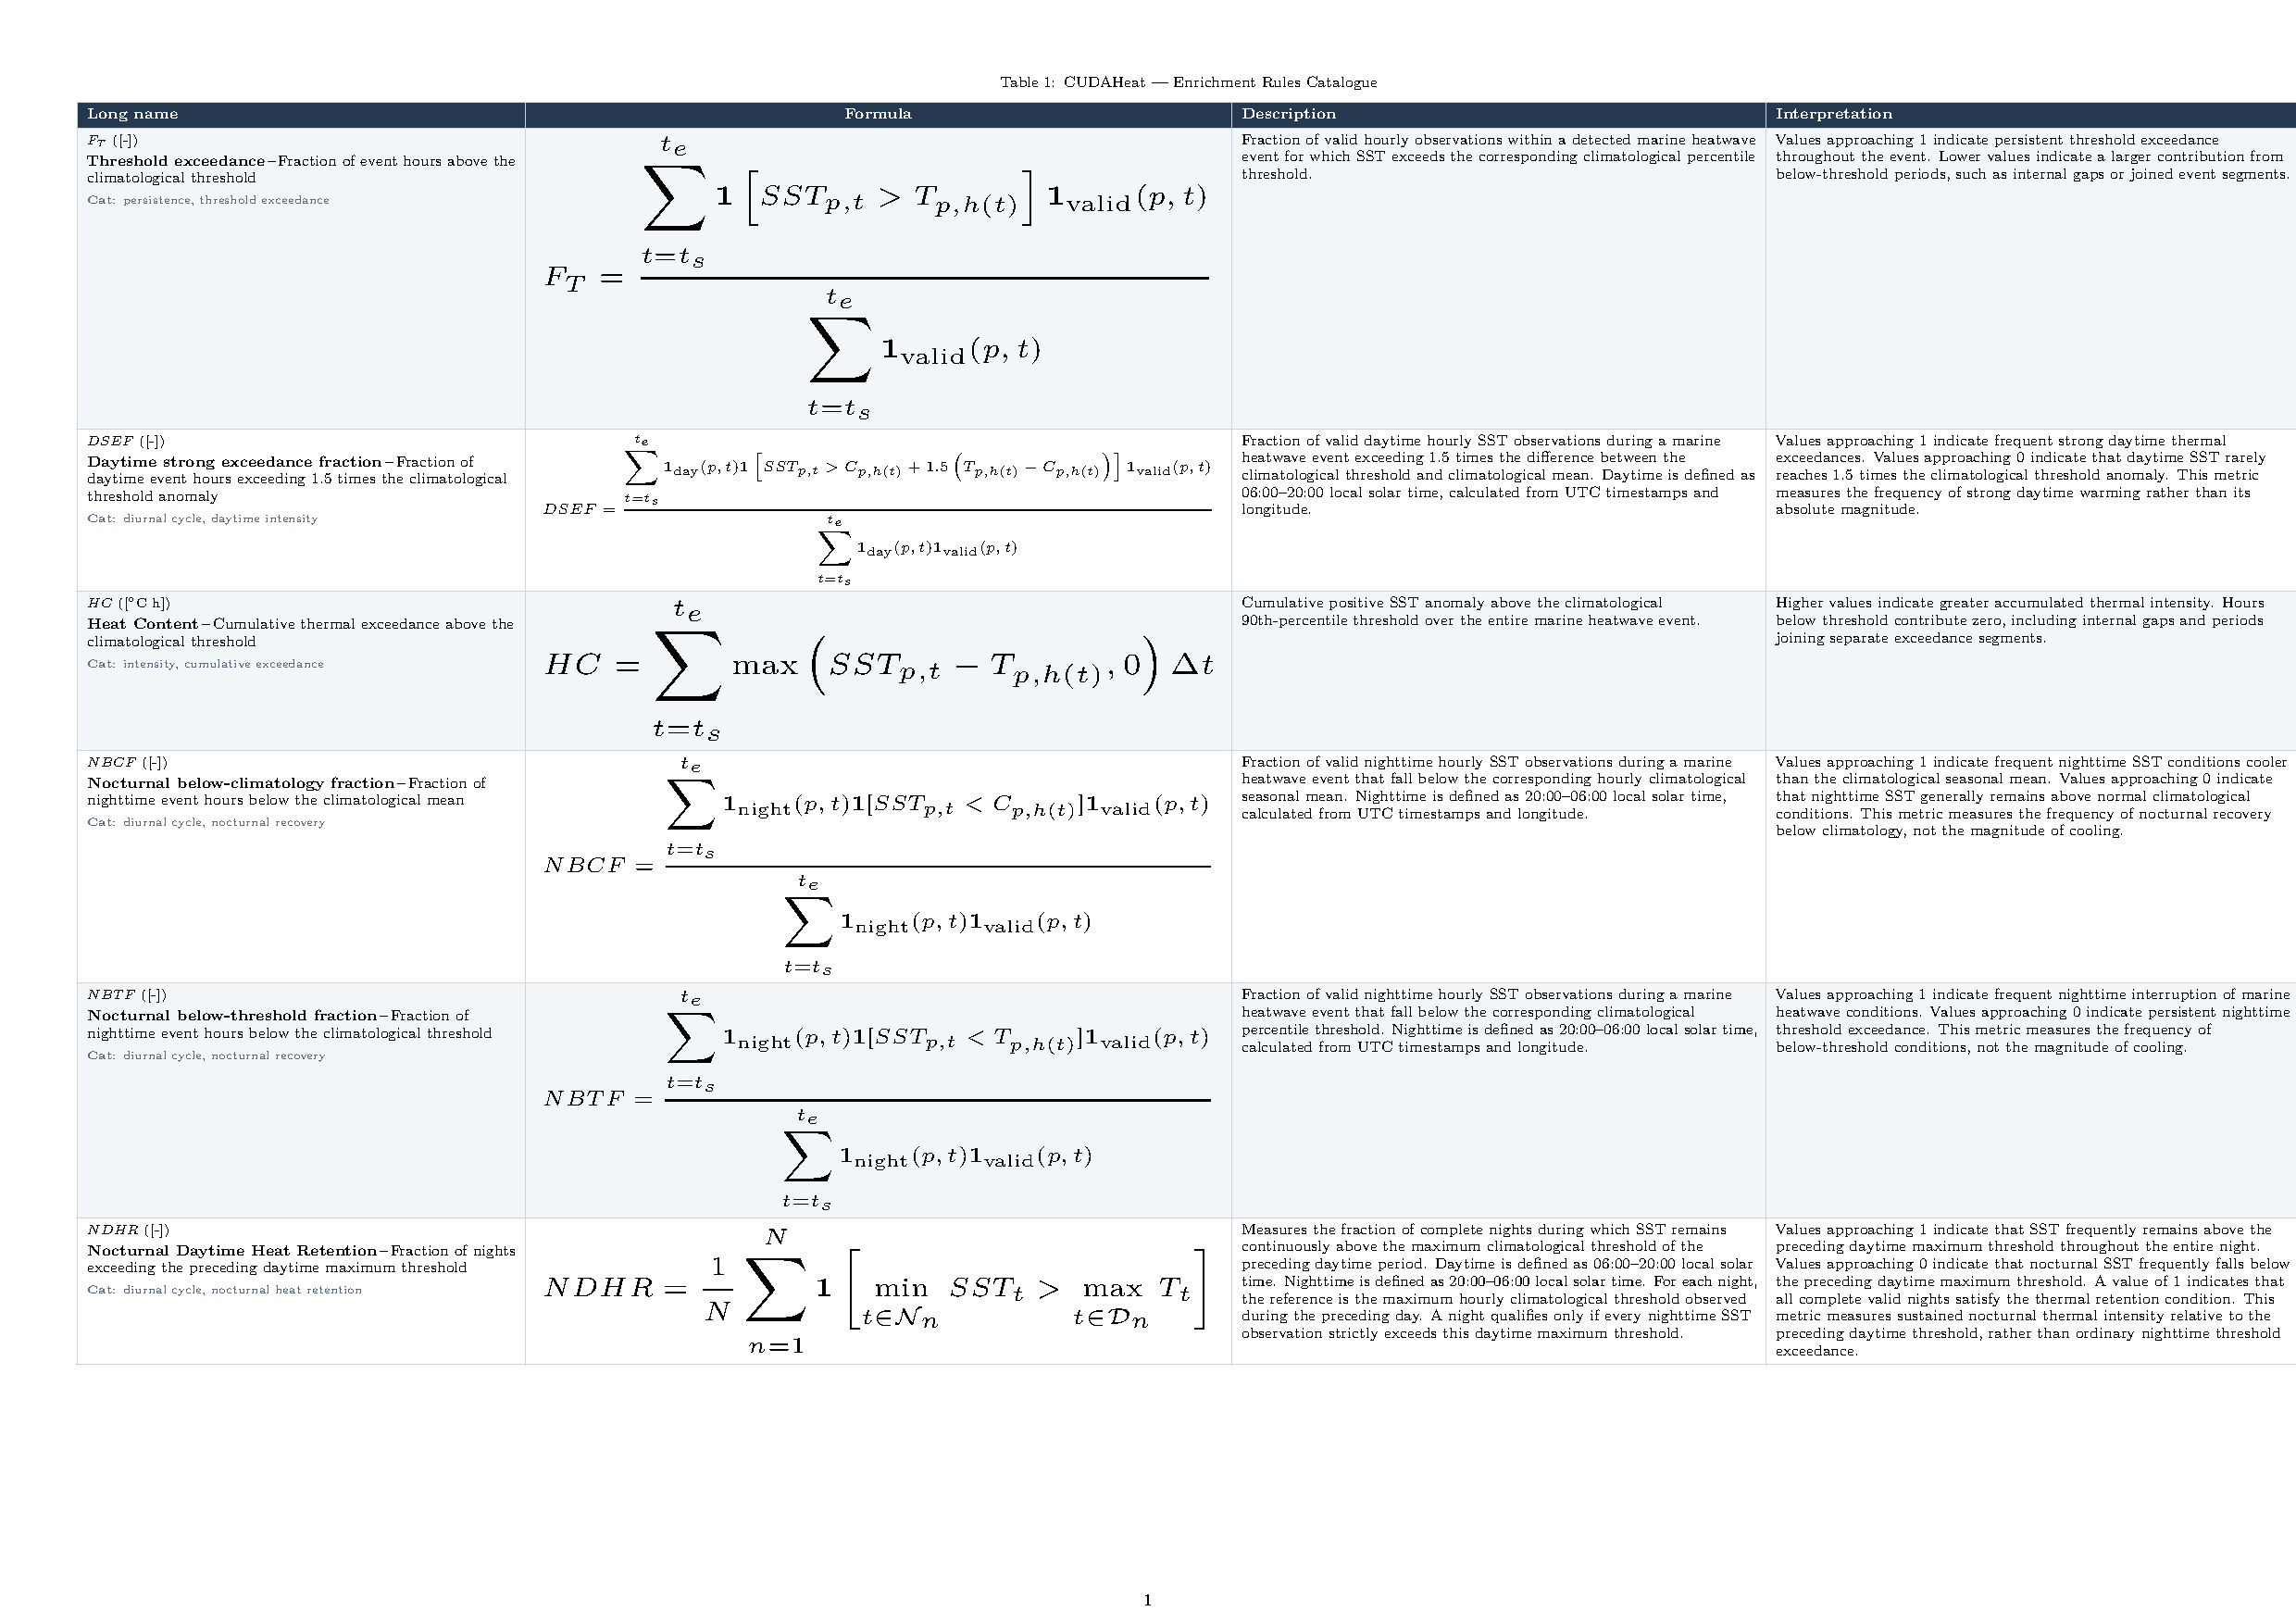
\includepdf[
    pages=-,
    fitpaper=true,
    pagecommand={\thispagestyle{plain}}
]{../examples/rule_laboratory/create_Table/create_Latex_table.pdf}
\clearpage

\subsection{Rule Evaluation}

\noindent\textbf{Integrated and standalone enrichment.}

Integrated enrichment is invoked during \code{detect()} and evaluates rules on device-resident batches after final event intervals have been determined. This avoids a second read of SST and annual-cycle fields. The standalone \code{enrich()} path supports retrospective application of rules to an existing sparse result. It reads the optimized source and cached cycles in storage-local batches, constructs aligned fields only when requested and evaluates interval reductions without iterating over individual events in Python.

Because a YAML rule embeds executable Python, rule directories are trusted extensions of the analysis environment. Schema validation confirms structure and declared metadata; it cannot establish scientific validity or prevent intentional side effects in arbitrary code. Reproducible use therefore requires version control of the rule directory, review of the embedded calculation and preservation of the recorded rule hashes.

\noindent\textbf{Rule provenance and event-aligned outputs.}

Rule outputs are attached to the sparse event catalogue using stable output names. The result metadata records the identifier, version, path, hash, formula and output declaration for every evaluated rule, together with enrichment timing information. This provenance permits a table of event descriptors to be traced back to the exact algorithm and configuration used for its production. It also makes it possible to repeat an enrichment analysis after a rule revision without overwriting or ambiguously merging measurements from different rule versions.

\clearpage
\section{Results}

\subsection{Hourly Event Detection}

%The primary result of CUDAHeat is a timestamp-resolved event catalogue whose boundaries are determined from the hourly threshold relation and declared continuity parameters. For every spatial point, the catalogue stores the start and stop indices, start and end times, duration and event identifier; the result metadata retains the baseline, percentile, smoothing window, calendar mode and gap parameters. This representation makes the assumptions that determine an event boundary explicit and permits the same SST record to be re-analysed under alternative scientifically motivated parameter choices.

%The hourly formulation resolves information that is unavailable after daily aggregation. The raw exceedance mask identifies the timing of threshold crossing, whereas the final interval records the continuity decision after short gaps, duration filtering and joining have been applied. These are distinct products. Reporting both the detection parameters and whether a subsequent metric is based on raw exceedance or final event membership is therefore necessary for an interpretable comparison of hourly marine heatwaves.

\subsection{Taxonomic Classification}

%Application of the enrichment catalogue produces event-aligned descriptors in the same sparse dataset as the event intervals. The resulting table can distinguish events with comparable duration but different sub-daily structure: for example, a high daytime strong-exceedance fraction may occur with frequent nocturnal recovery, while sustained nocturnal retention may occur without an equally large daytime peak. Heat-content and threshold-exceedance measures provide complementary information about cumulative thermal forcing and temporal occupancy above threshold.

%The taxonomic result is deliberately multivariate. CUDAHeat does not assign a single categorical label unless such a classification is introduced by a subsequent analysis. Instead, the rule outputs provide a transparent feature space in which regional, ecological or process-based hypotheses can be tested. This avoids treating a software-level descriptor catalogue as evidence for a universal partition of marine heatwaves.

\subsection{Feature-Space Results and Scatterplot Representation}

%Scatterplots should treat each retained event as one observation in the declared descriptor space. Direct metric--metric plots retain physical units and are suitable when the relationship between two named scalars is the subject of inference. When a PCA projection is shown, the axes should be labelled as component scores, not as raw physical variables; the accompanying analysis should report the loadings and explained variance. A third descriptor may be represented by colour, symbol shape or faceting only when its scale, normalization and missing-data treatment are stated explicitly.

%Overplotting can obscure the distribution of large event catalogues. Transparency, density estimates, hexagonal binning or stratified sampling may be used for visualization, but the population represented by the graphic must remain identifiable. Scatterplot separation alone should not be interpreted as a physically distinct class: apparent clusters may arise from scaling, correlated descriptors, sampling density or the event-selection rule. The raw rule outputs and the normalization parameters should therefore be retained with any PCA scores or graphical products.

\subsection{Case Studies}

%At event scale, \code{event_timeseries()} returns a padded time window containing SST, climatology, threshold, raw exceedance and event identifiers. These fields allow onset, interruption and termination to be inspected against the diurnally resolved reference state. At point scale, \code{point_timeseries()} and \code{point_events()} provide the corresponding local history and catalogue subset. Together, these products support case studies in which the event boundary and the derived taxonomy can be examined before they are aggregated spatially or temporally.

%For regional analyses, the sparse catalogue can be filtered by date, duration or point index and reconstructed lazily only where a dense map is needed. The recommended reporting unit is therefore not solely an event count: it is the combination of source product, hourly climatology definition, detection configuration and versioned enrichment rules. This combination provides the context required to compare case studies without conflating differences in scientific definition with differences in observed thermal behaviour.

\clearpage

\input{tikz/test/event-000001_point-0}
\input{tikz/test/event-000002_point-0}

\input{tikz/test/event-000011_point-0}
\input{tikz/test/event-000012_point-0}
\input{tikz/test/event-000013_point-0}
\input{tikz/test/event-000015_point-0}
\input{tikz/test/event-000020_point-0}
\input{tikz/test/event-000023_point-0}
\input{tikz/test/event-000024_point-0}

\clearpage
\section{Conclusions}

%CUDAHeat provides a reproducible framework for moving marine-heatwave analysis from daily aggregates to hourly SST records. Its defining methodological choice is to preserve every time step for each spatial point while batching only across space. This allows an hourly climatology, a same-hour percentile threshold and temporal continuity rules to be evaluated without changing the time series at batch boundaries.

%The framework returns sparse, queryable event catalogues and a versioned set of event-aligned descriptors. By separating threshold construction, event detection and enrichment, it makes the assumptions underlying an hourly marine heatwave visible and revisable. The resulting workflow is intended to support scientifically explicit analysis of diurnal structure, nocturnal recovery, thermal persistence and cumulative exceedance in gridded SST products.

\clearpage
% \appendix
% %\section{Public API Reference}

%The principal entry point is \code{CUDAHeat(source, variable=...)}. The \code{run()} method computes requested fields, whereas \code{detect()} returns an \code{EventDetectionResult}. Convenience methods expose the smoothed climatology, aligned threshold and in-memory exceedance mask. The result object supplies event selection, point-level catalogues, point time series, event-centred time series and lazy dense reconstruction. Numerical diagnostics are available through \code{validate()}, which compares CPU reference fields and GPU fields using the same temporal formulation.

% %\section{Enrichment Rule Schema}

%An enrichment rule declares an identifier, version, names, symbol, category, description, interpretation, mathematical formula, symbol dictionary and output specification, together with executable Python. The output specification requires a name, unit, range and dimensions. Rules are discovered from YAML files, schema-validated, compiled and identified by both semantic version and source hash. Rules should be treated as trusted, version-controlled scientific software.

% %\section{Configuration Reference}

%The detection definition comprises the source variable, baseline interval, percentile, calendar mode, smoothing choices, minimum duration, internal-gap allowance and joining allowance.

%The execution configuration comprises precision, VRAM reserve, batch selection and input-optimization policy. Optional persistence is configured through a PostgreSQL INI file whose credentials are resolved from the environment or standard \code{libpq} configuration. All parameters that define detection or enrichment are retained in result metadata.




%\printcredits

%% Loading bibliography style file


% Loading bibliography database
\bibliographystyle{class/cas-model2-names}
\bibliography{class/cas-refs}


%\vskip3pt

% \bio{}
% Author biography without author photo.
% Author biography. Author biography. Author biography.
% Author biography. Author biography. Author biography.
% Author biography. Author biography. Author biography.
% Author biography. Author biography. Author biography.
% Author biography. Author biography. Author biography.
% Author biography. Author biography. Author biography.
% Author biography. Author biography. Author biography.
% Author biography. Author biography. Author biography.
% Author biography. Author biography. Author biography.
% \endbio

% \bio{}
% Author biography with author photo.
% Author biography. Author biography. Author biography.
% Author biography. Author biography. Author biography.
% Author biography. Author biography. Author biography.
% Author biography. Author biography. Author biography.
% Author biography. Author biography. Author biography.
% Author biography. Author biography. Author biography.
% Author biography. Author biography. Author biography.
% Author biography. Author biography. Author biography.
% Author biography. Author biography. Author biography.
% \endbio

% \bio{}
% Author biography with author photo.
% Author biography. Author biography. Author biography.
% Author biography. Author biography. Author biography.
% Author biography. Author biography. Author biography.
% Author biography. Author biography. Author biography.
% \endbio

\end{document}
